\begin{tikzpicture}[x=1cm, y=1cm, font=\sffamily\footnotesize,
  ptitle/.style={anchor=west, font=\sffamily\bfseries\small, text=narrareddeep},
  textbox/.style={draw=phaseA!60, fill=phaseA!6, rounded corners=2pt, inner sep=4pt, anchor=north west,
                  align=left, font=\sffamily\scriptsize},
  lbl/.style={draw=#1, fill=white, fill opacity=0.9, text opacity=1, rounded corners=1pt, inner sep=1.6pt,
              line width=0.6pt, font=\sffamily\scriptsize},
  lblkey/.style={draw=#1, fill=white, fill opacity=0.95, text opacity=1, rounded corners=1pt, inner sep=1.8pt,
                 line width=1.0pt, font=\sffamily\scriptsize\bfseries},
  lead/.style={draw=#1, line width=0.7pt},
  path/.style={-{Latex[length=2.6mm, width=2.4mm]}, draw=black!85, line width=1.6pt},
  imgcap/.style={anchor=north, font=\sffamily\scriptsize, text=black!60},
  chip/.style={draw=black!30, fill=white, rounded corners=6pt, inner sep=2.5pt, font=\sffamily\footnotesize},
  flow/.style={-{Latex[length=1.6mm]}, draw=black!50, line width=0.6pt},
  lab/.style={anchor=east, font=\sffamily\footnotesize, text=black!75},
  txt/.style={anchor=west, font=\sffamily\footnotesize, text=black!75}]

\node[ptitle] at (0,0.000) {(a) An example task of this family and its room (AI2-THOR rendering)};
\node[textbox, text width=14.70cm] (obs) at (0,-0.280) {\textbf{Goal.} Your task is to: examine the book with the desklamp.\\[1pt]\textbf{Initial observation.} You are in the middle of a room. Looking quickly around you, you see a bed 1, a desk 2, a desk 1, a drawer 6, a drawer 5, a drawer 4, a drawer 3, a drawer 2, a drawer 1, a garbagecan 1, a laundryhamper 1, a safe 1, a shelf 6, a shelf 5, a shelf 4, a shelf 3, a shelf 2, and a shelf 1.};
\begin{scope}[shift={($(obs.south west)+(0,-0.25)$)}]
\node[anchor=north west, inner sep=0] at (0.000,0.000) {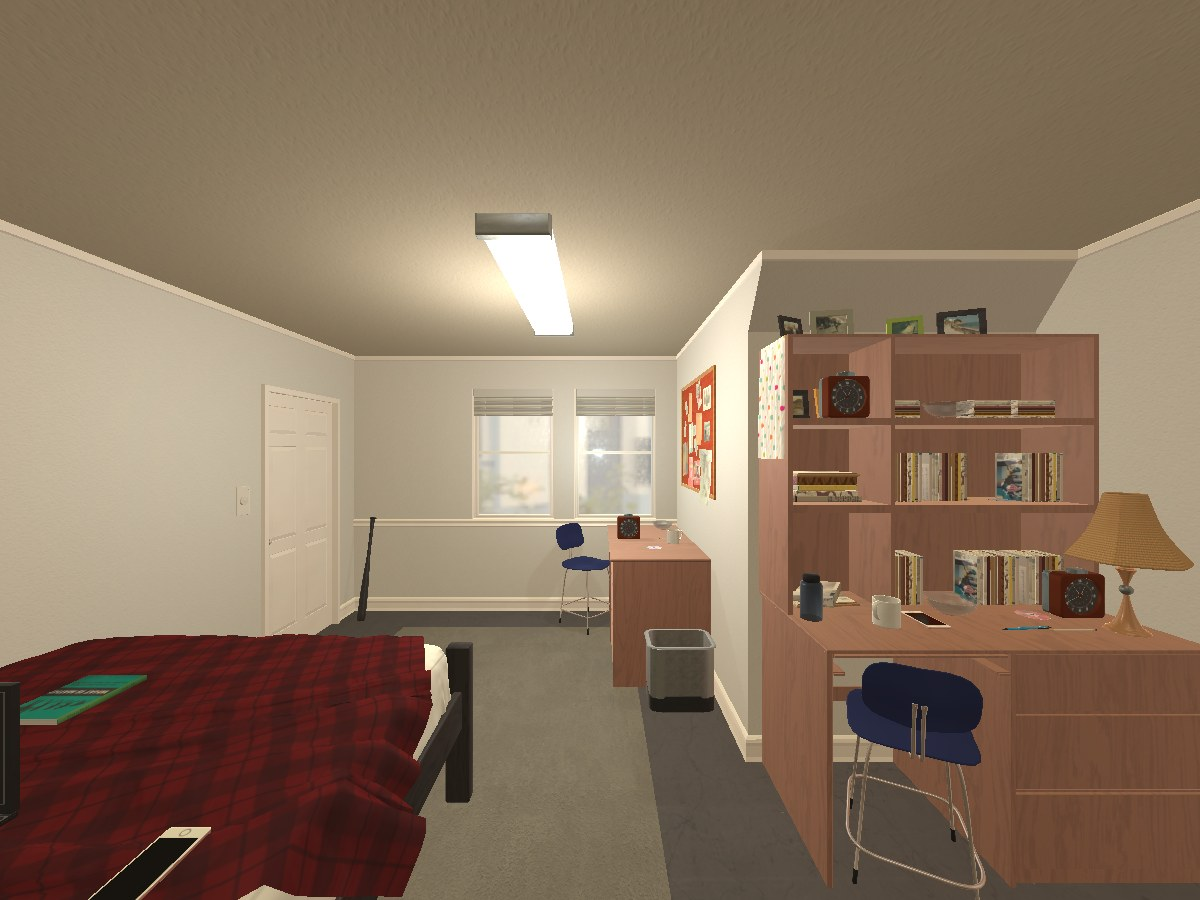
\includegraphics[width=8.487cm]{figures/cases/examine_view1.jpg}};
\draw[black!35, line width=0.4pt] (0.000,0.000) rectangle ++(8.487,-6.365);
\draw[dimF, line width=1.1pt] (0.587,-4.954) circle (0.535);
\draw[lead=dimF] (0.587,-4.954) -- (0.587,-4.454);
\fill[dimF] (0.587,-4.954) circle (0.06);
\node[lblkey=dimF] at (0.587,-4.454) {book};
\draw[dimA, line width=1.1pt, rounded corners=1pt] (0.000,-4.491) rectangle (3.338,-6.365);
\fill[dimA] (1.669,-5.428) circle (0.06);
\node[lblkey=dimA] at (1.669,-5.428) {bed: the book is here};
\draw[dimE, line width=1.1pt, rounded corners=1pt] (7.525,-3.487) rectangle (8.438,-4.512);
\draw[lead=dimE] (7.981,-4.000) -- (6.988,-3.646);
\fill[dimE] (7.981,-4.000) circle (0.06);
\node[lblkey=dimE] at (6.988,-3.646) {desklamp: turn it on};
\fill[black!55] (6.928,-5.234) circle (0.06);
\node[lbl=black!45] at (6.928,-5.234) {desks};
\draw[lead=black!55] (7.030,-3.989) -- (6.130,-4.180);
\fill[black!55] (7.030,-3.989) circle (0.06);
\node[lbl=black!45] at (6.130,-4.180) {shelves};
\draw[lead=black!55] (7.833,-5.877) -- (6.933,-5.686);
\fill[black!55] (7.833,-5.877) circle (0.06);
\node[lbl=black!45] at (6.933,-5.686) {drawers};
\node[anchor=north west, inner sep=0] at (8.737,0.000) {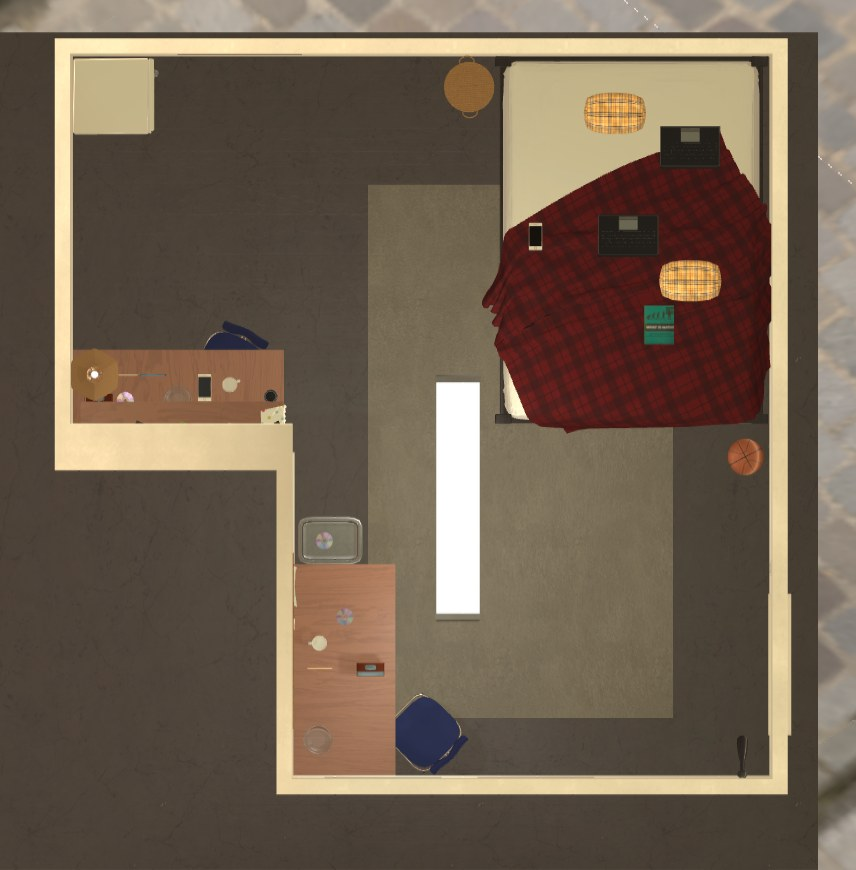
\includegraphics[width=6.263cm]{figures/cases/examine_map.jpg}};
\draw[black!35, line width=0.4pt] (8.737,0.000) rectangle ++(6.263,-6.365);
\fill[black, opacity=0.22] (11.708,-0.789) -- ++(-135:1.1) arc (-135:-45:1.1) -- cycle;
\fill[black] (11.708,-0.789) circle (0.08);
\draw[white, line width=3.4pt, opacity=0.85] (13.163,-1.765) -- (9.665,-2.678);
\draw[path] (13.163,-1.765) -- (9.665,-2.678);
\draw[lead=dimA] (13.357,-1.715) -- (13.357,-1.215);
\fill[dimA] (13.357,-1.715) circle (0.06);
\node[lblkey=dimA] at (13.357,-1.215) {bed: the book is here};
\draw[lead=dimE] (9.423,-2.741) -- (10.416,-3.094);
\fill[dimE] (9.423,-2.741) circle (0.06);
\node[lblkey=dimE] at (10.416,-3.094) {desklamp: turn it on};
\draw[lead=black!55] (10.223,-2.835) -- (10.223,-2.335);
\fill[black!55] (10.223,-2.835) circle (0.06);
\node[lbl=black!45] at (10.223,-2.335) {desk};
\draw[lead=black!55] (11.356,-5.082) -- (11.356,-4.582);
\fill[black!55] (11.356,-5.082) circle (0.06);
\node[lbl=black!45] at (11.356,-4.582) {desk};
\draw[lead=black!55] (9.672,-2.767) -- (9.291,-2.028);
\fill[black!55] (9.672,-2.767) circle (0.06);
\node[lbl=black!45] at (9.291,-2.028) {drawers};
\draw[lead=black!55] (11.424,-4.531) -- (11.424,-4.031);
\fill[black!55] (11.424,-4.531) circle (0.06);
\node[lbl=black!45] at (11.424,-4.031) {drawers};
\draw[lead=black!55] (11.153,-3.956) -- (10.454,-3.602);
\fill[black!55] (11.153,-3.956) circle (0.06);
\node[lbl=black!45] at (10.454,-3.602) {garbagecan};
\draw[lead=black!55] (12.169,-0.637) -- (11.382,-0.283);
\fill[black!55] (12.169,-0.637) circle (0.06);
\node[lbl=black!45] at (11.382,-0.283) {laundryhamper};
\draw[lead=black!55] (9.550,-0.704) -- (9.309,-0.242);
\fill[black!55] (9.550,-0.704) circle (0.06);
\node[lbl=black!45] at (9.309,-0.242) {safe};
\draw[lead=black!55] (10.174,-3.124) -- (9.678,-4.140);
\fill[black!55] (10.174,-3.124) circle (0.06);
\node[lbl=black!45] at (9.678,-4.140) {shelves};
\node[imgcap] at (4.244,-6.405) {first-person view inside the room};
\node[imgcap] at (11.869,-6.405) {the room from above; cone: the left view; arrow: the expert's route};
\node[anchor=west, font=\sffamily\bfseries\footnotesize, text=black!70] at (0,-7.165) {Expert solution (4 steps):};
\node[chip, anchor=west] (s0) at (3.900,-7.165) {go to bed};
\node[chip, anchor=west] (s1) at (5.878,-7.165) {take book from bed};
\draw[flow] (s0.east) -- (s1.west);
\node[chip, anchor=west] (s2) at (9.134,-7.165) {go to desk};
\draw[flow] (s1.east) -- (s2.west);
\node[chip, anchor=west] (s3) at (11.254,-7.165) {use desklamp};
\draw[flow] (s2.east) -- (s3.west);
\node[ptitle] at (0.000,-7.965) {(b) Effect of the memory on this family, 3 demonstration pairs};
\node[txt, text=black!65] at (0.000,-8.415) {family success: GPT $0.648\rightarrow0.833$, Qwen $0.611\rightarrow0.574$};
\draw[black!45] (7.400,-8.815) -- (7.400,-10.945);
\node[font=\sffamily\scriptsize, text=black!50] at (5.000,-11.115) {$-1$};
\node[font=\sffamily\scriptsize, text=black!50] at (7.400,-11.115) {$0$};
\node[font=\sffamily\scriptsize, text=black!50] at (9.800,-11.115) {$+1$};
\node[lab] at (4.850,-9.085) {task 7};
\fill[gptblue!55] (7.400,-8.935) rectangle ++(1.601,-0.24);
\node[anchor=west, font=\sffamily\scriptsize, text=black!70] at (9.061,-9.055) {$+0.667$};
\fill[qwenmint!55] (7.400,-9.225) rectangle ++(0.799,-0.24);
\node[anchor=west, font=\sffamily\scriptsize, text=black!70] at (8.259,-9.345) {$+0.333$};
\node[lab] at (4.850,-9.745) {task 45};
\fill[gptblue!55] (7.400,-9.595) rectangle ++(1.601,-0.24);
\node[anchor=west, font=\sffamily\scriptsize, text=black!70] at (9.061,-9.715) {$+0.667$};
\fill[qwenmint!55] (7.400,-9.885) rectangle ++(-1.601,-0.24);
\node[anchor=east, font=\sffamily\scriptsize, text=black!70] at (5.739,-10.005) {$-0.667$};
\node[lab] at (4.850,-10.405) {task 89};
\fill[gptblue!55] (7.400,-10.255) rectangle ++(-1.200,-0.24);
\node[anchor=east, font=\sffamily\scriptsize, text=black!70] at (6.140,-10.375) {$-0.500$};
\fill[qwenmint!55] (7.400,-10.545) rectangle ++(0.000,-0.24);
\node[anchor=west, font=\sffamily\scriptsize, text=black!70] at (7.460,-10.665) {$0$};
\fill[gptblue!55] (0.000,-9.165) rectangle ++(0.28,-0.18);
\node[txt] at (0.320,-9.255) {GPT-4o-mini};
\fill[qwenmint!55] (0.000,-9.565) rectangle ++(0.28,-0.18);
\node[txt] at (0.320,-9.655) {Qwen3-8B};
\end{scope}
\end{tikzpicture}
